\documentclass{article}
\usepackage[svgnames]{xcolor}
\usepackage{tikz}
\usepackage{verbatim}
\usetikzlibrary{perspective}

\begin{document}
\usetikzlibrary {perspective}

\newcommand{\simpleaxes}[3]{%
\draw[->] (-0.5,0,0) -- (#1,0,0) node[pos=1.1]{x};
\draw[->] (0,-0.5,0) -- (0,#2,0) node[pos=1.1]{y};
\draw[->] (0,0,-0.5) -- (0,0,#3) node[pos=1.1]{z};}

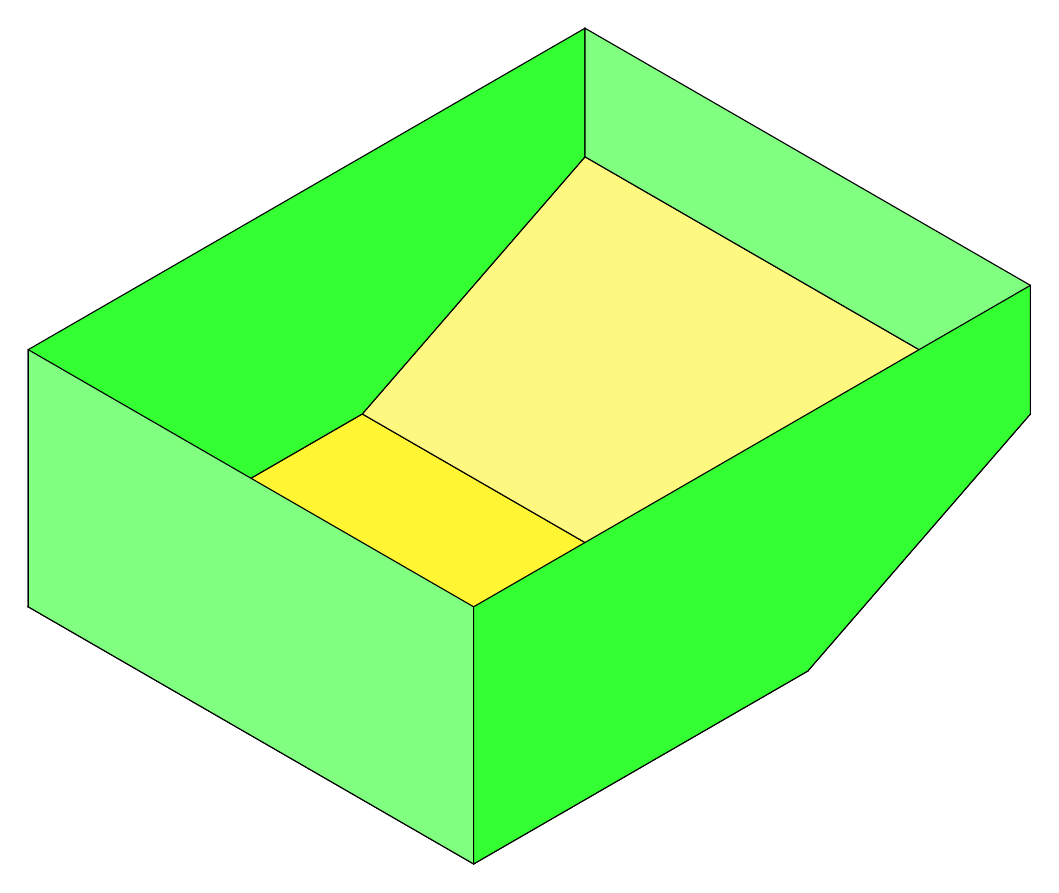
\begin{tikzpicture}[
  scale=1.0,
  isometric view
  ]

\filldraw[fill=yellow!80!white] (tpp cs:x=0,y=0,z=0)
-- (tpp cs:x=6,y=0,z=0)
-- (tpp cs:x=6,y=8,z=0)
-- (tpp cs:x=0,y=8,z=0) -- cycle;

\filldraw[fill=yellow!50!white] (tpp cs:x=6,y=0,z=0)
-- (tpp cs:x=10,y=0,z=2)
-- (tpp cs:x=10,y=8,z=2)
-- (tpp cs:x=6,y=8,z=0) -- cycle;

\filldraw[fill=green!80!white] (tpp cs:x=0,y=8,z=0)
-- (tpp cs:x=6,y=8,z=0)
-- (tpp cs:x=10,y=8,z=2)
-- (tpp cs:x=10,y=8,z=4)
-- (tpp cs:x=0,y=8,z=4) -- cycle;

\filldraw[fill=green!50!white] (tpp cs:x=10,y=8,z=2)
-- (tpp cs:x=10,y=0,z=2)
-- (tpp cs:x=10,y=0,z=4)
-- (tpp cs:x=10,y=8,z=4) -- cycle;

\filldraw[fill=green!50!white] (tpp cs:x=0,y=8,z=0)
-- (tpp cs:x=0,y=0,z=0)
-- (tpp cs:x=0,y=0,z=4)
-- (tpp cs:x=0,y=8,z=4) -- cycle;

\filldraw[fill=green!80!white] (tpp cs:x=0,y=0,z=0)
-- (tpp cs:x=6,y=0,z=0)
-- (tpp cs:x=10,y=0,z=2)
-- (tpp cs:x=10,y=0,z=4)
-- (tpp cs:x=0,y=0,z=4) -- cycle;

\end{tikzpicture}
\end{document}

